\section{The SegmentAnalyser class} \label{sec:sa}

\subsection{Analysis per segment, rootsystem length density}

The class SegmentAnalyser offers post-processing methods per root segment. The advantage is that we can do distributions or densities, and that we can crop the segments with any geometry. 

We start with a small example plotting the root surface densities of a root system versus root depth.

\lstinputlisting[language=Python, caption=Example 3a]{../../examples/python/example3a_density.py}

\begin{figure}
\centering
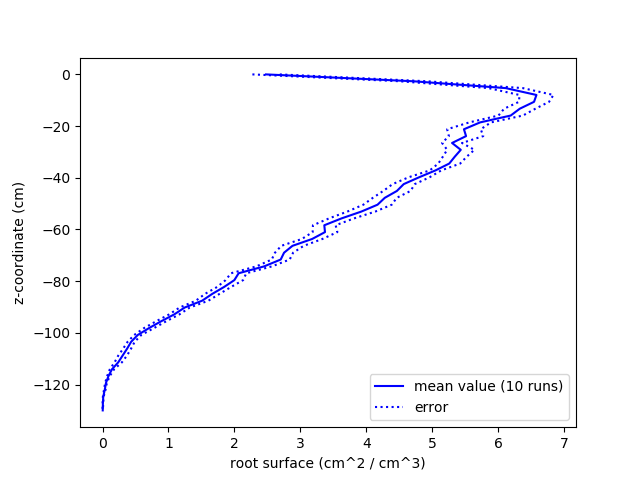
\includegraphics[width=0.7\textwidth]{example_3c.png}
\caption{Root surface densitiy versus depth mean (Example 3a), and standard error ($N$=10)} \label{fig:surface_density}
\end{figure}


\begin{itemize}

\item[8-12] Pick a root system.
\item[14-16] Depth describes the y-axis of the graph, layers the number of vertical soil layers, where the root surface is accumulated, and runs is the number of simulation runs. 
\item[18-23] Perfoms the simulations. L23 creates a distribution of a parameter (name) over a vertical range (bot, top). The data are accumulated layers, segments are either cut (exact = True) or accumaled by their mid point (exact = False). 
\item[25] In order to calculate a root surface density from the summed up surface, we need to define a soil volume. The vertical height is the layer length, lenght and widht (here 10 cm), can be determined by planting widht, or by geometry, if root growth is confined. 
\item[26-28] Calculates the densitis, mean densities, and standard error. 
\item[30-39] Prepares teh plot (see Figure \ref{fig:surface_density}).

\end{itemize}



\subsection{Analysis per segment using SDF}

The following script demonstrates some of the post processing possibilities by setting up a virtual soil core experiment, where we analyse the content of two soil cores located at other positions.

\lstinputlisting[language=Python, caption=Example 3b]{../../examples/python/example3b_sdfanalysis.py}

\begin{itemize}

\item[9-15] Performs the simulation.

\item[17-20] We define two soil cores, one in the center of the root and one 10 cm translated. In L16 we pick which one we use for the further analysis.  Figure \ref{fig:soilcoreGeom} shows the resulting geometry.

\item[23] We pick which geometry we will use for further analysis.

\item[25-29] Prepares the plot. We use four sub-figures. 

\item[31-35] Creates a root length distribution versus depth. L32 creates the SegmentAnalyser object, and L41 creates the distribution.

\item[37-43] Performs the same distribution in the soil core. In L39 we crop the segments to the geometry. L49 is used to delete unused nodes. 

\item[45-52] Same as before, but we are only interested in segments that are younger than 30 days. In L47 we use the filer method (name, min, max) to keep only the segments we want in the analysis. 

\item[54-61] The filter method can be used for many different applications. In the following we use it to analyse lateral roots only. Possible rb.ScalarType are: 'type', 'radius', 'order', segment creation time 'time', 'length', 'surface', 'volume', 'one', 'userdata1', 'userdata2', 'userdata3', and 'parenttype'.

\item[63-65] Show and save resulting Figure \ref{fig:central}, and \ref{fig:shifted}.

\end{itemize}

In this example the central core captures only a little amount of laterals (Figure \ref{fig:central}) because the root system is wide spread. 
The shifted root core represents the overall root system slightly better, see Figure \ref{fig:shifted}.  
The basic idea is that such simulations help to increase the understanding of experimental observations.

\begin{figure}
\centering
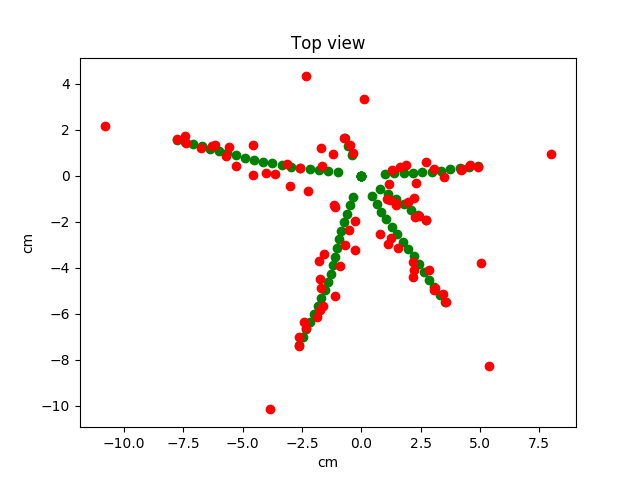
\includegraphics[width=0.7\textwidth]{example_3d.png} % 
\caption{Virtual soil cores experiment (Example 3b): Central core (blue), shifted core (red)} \label{fig:soilcoreGeom}
\end{figure} 

\begin{figure}
\centering
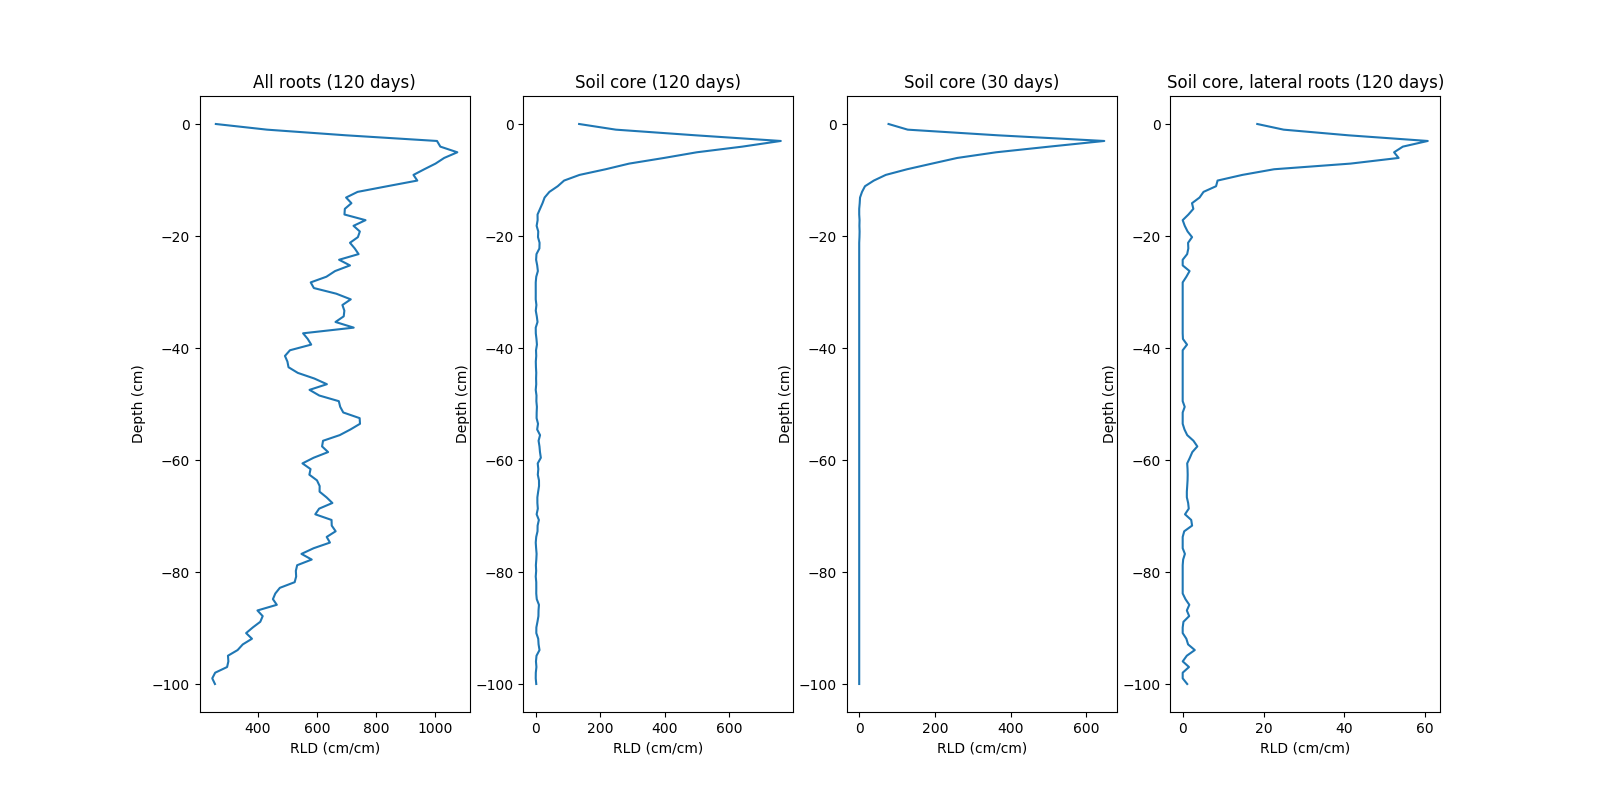
\includegraphics[width=0.9\textwidth]{example_3d1.png} 
\caption{Central core (Example 3b)} \label{fig:central}
\end{figure}

\begin{figure}
\centering
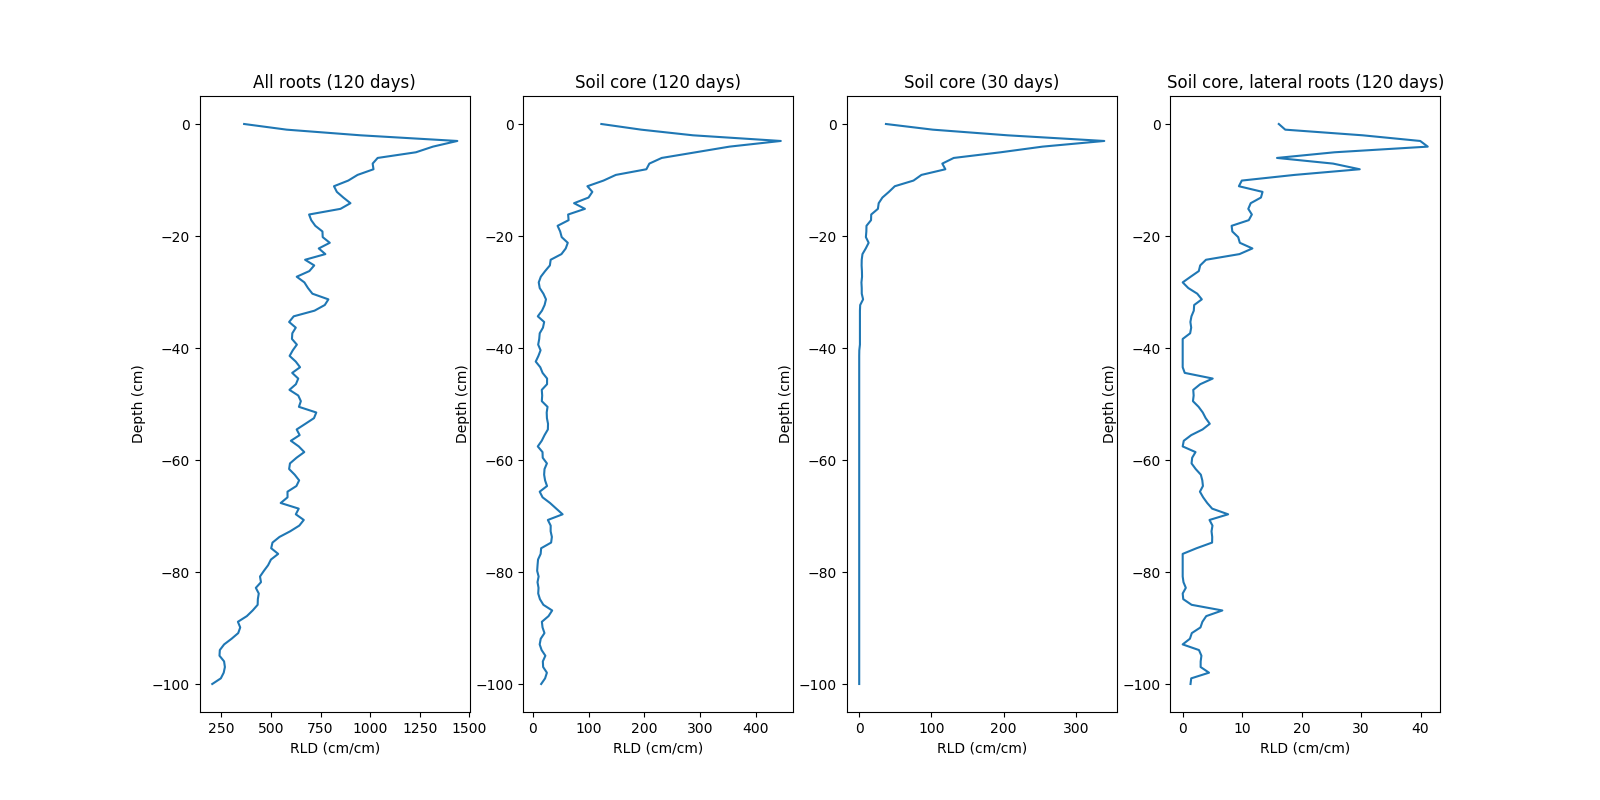
\includegraphics[width=0.9\textwidth]{example_3d2.png} 
\caption{Shifted core (Example 3b)} \label{fig:shifted}
\end{figure}


\subsection{SegmentAnalyser for DGF or VTP export}

If we want to export our root system as dune grid file (dgf) we need to introduce an artificial shoot. By default the tap root and basal root starts at the seed node (i.e. multiple segments start at the same node), and its difficult to define a boundary condition in Dumux for such a situation. Furthermore, if there are shoot borne roots, they emerge out of nothing above the seed node. Therefore, we introduce artifical segments eventually connecting shoot borne roots (if there are any) and connecting the seed node (noramlly located at 0,0,-3) to the orgin at (0,0,0). The following code snippet shows how to export a RootSytem dgf:

\lstinputlisting[language=Python, caption=Example 3c]{../../examples/python/example3c_write.py}

\begin{itemize}
 \item[6-11] Define a example root sytemytem
 \item[13] Create the analyser object
 \item[15-18] Get the artificial shoot segments from the root sytem (L15) and manually add them ot the SegmentAnalyser (L18).
 \item[20] Write the DGF file 
\end{itemize}

It is also possible to make use of the SegmentAnalyser class without any ohter CPlantBox classes (e.g. for writing vtp from measurements). The following example shows how to construct the class with arbitrary nodes and segments (e.g. from measurements). 

\lstinputlisting[language=Python, caption=Example 3d]{../../examples/python/example3d_measurements.py}

\begin{itemize}
 \item[6-9] Define some segments with data
 \item[14,15] We convert the Python list to lists of C++ types
 \item[20] We create the SegmentAnalyser object without an underlying Organsim
\end{itemize}



In the following we show how model parameters can be modified, and how a sensitivity analysis can be performed. Additionally, we comment on how to best make an animation from a CPlantBox simulation.





\subsection{How to make an animation}

In order to create an animation in Paraview we have to consider some details. The main idea is to export the result file as segments using the class SegmentAnalyser. A specific frame is then obtained by thresholding within Paraview using the segments creation times. 

We modify example1b.py to demonstrate how to create an animation.

%\lstinputlisting[language=Python, caption=Example 4c (modified from Example 1b)]{../../examples/python/example4c.py} 

\begin{itemize}

\item[17,18] Its important to use a small resolution in order to obtain a smooth animation. L18 set the axial resolution to 0.1 cm. 

\item[25] Instead of saving the root system as polylines, we use the SegmentAnalyser to save the root system as segments.

\item[28] We save the geometry as Python script for the visualization in ParaView.

\end{itemize}

After running the script we perform the following operations to create an animation:
\begin{enumerate}
 \item Open the .vtp file in ParaView (File$\rightarrow$Open...), and open tutorial/examples/python/results/example\_4c.vtp.
 \item Optionally, create a tube plot with the help of the script tutorial/pyscript/rsTubePlot.py (Tools$\rightarrow$Python Shell, press 'Run script').
 \item Run the script tutorial/pyscript/rsAnimate.py (Tools$\rightarrow$Python Shell, press 'Run script'). The script creates the threshold filter and the animation. 
 \item Optionally, visualize the domain boundaries by running the script tutorial/examples/python/results/example\_4c.py (Tools$\rightarrow$Python Shell, press 'Run script'). Run after the animation script (ohterwise it does not work).  
 \item Use File$\rightarrow$Save Animation... to render and save the animation. Pick quality (<100 \%), and the frame rate in order to achieve an appropriate video length, e.g. 300 frames with 50 fps equals 6 seconds. Files might be very big, and needs compression (e.g. ffmpeg -i in.avi -vcodec libx264 -b 4000k -an out.avi, produces high quality, tiny file size, and plays with VLC).
\end{enumerate}




